\documentclass{beamer}
\usepackage[utf8]{inputenc}
\usepackage[backend=biber,style=alphabetic,sorting=ynt]{biblatex}
\addbibresource{mybib.bib}

\usepackage{tikz}
\usetikzlibrary{positioning}

\mode<presentation> {
\usetheme{Madrid}
}

\usecolortheme{default}

%------------------------------------------------------------
%This block of code defines the information to appear in the
%Title page
\title[C*-algebras and K-theory] %optional
{C*-algebras and K-theory for Infinite Dimensional Hilbert Manifolds}\label{titlepage}

%\subtitle{A short story}
\author[Abdul Halim] 
{Abdul Halim\inst{1}}
\institute[] 
{
  \inst{1}
 \texttt{abdul.halim@uni-goettingen.de}
}
\date[] 
{\large \textbf{Mathematisches Institut}}
\titlegraphic{\includegraphics[height=3.0cm]{uni-goettingen-logo.jpg}}


%End of title page configuration block
%------------------------------------------------------------

% Customizing the footer
\setbeamertemplate{footline}
{
  \leavevmode%
  \hbox{%
    \begin{beamercolorbox}[wd=.2\paperwidth,ht=3ex,dp=1.5ex,leftskip=1em,center]{author in head/foot}%
      \usebeamerfont{author in head/foot}Abdul Halim
    \end{beamercolorbox}%
    \begin{beamercolorbox}[wd=.6\paperwidth,ht=3ex,dp=1.5ex,center]{title in head/foot}%
      \usebeamerfont{title in head/foot}C*-algebras and K-theory for Infinite Dimensional Hilbert Manifolds
    \end{beamercolorbox}%
    \begin{beamercolorbox}[wd=.2\paperwidth,ht=3ex,dp=1.5ex,rightskip=1em,center]{date in head/foot}%
      \usebeamerfont{date in head/foot}\insertframenumber/\inserttotalframenumber
    \end{beamercolorbox}%
  }%
  \vskip0pt%
}

%------------------------------------------------------------
%The next block of commands puts the table of contents at the 
%beginning of each section and highlights the current section:

\AtBeginSection[]
{
  \begin{frame}
    \frametitle{Table of Contents}
    \tableofcontents[currentsection]
  \end{frame}
}
%------------------------------------------------------------


\begin{document}

%The next statement creates the title page.
\frame{\titlepage}


%---------------------------------------------------------
%This block of code is for the table of contents after
%the title page
\begin{frame}
\frametitle{Table of Contents}
\tableofcontents
\end{frame}
%---------------------------------------------------------


\section{Introduction}

%---------------------------------------------------------
%Changing visivility of the text
\begin{frame}
\frametitle{Introduction}
\begin{center}
\begin{figure}[h!]
\includegraphics[width=0.5\textwidth]{manifold.png}
\caption{Idea of infinite dimensional manifold}
\end{figure}
\end{center}
In this research, we aim to explore the interplay between C*-algebras, K-theory, and Fredholm manifolds modeled on infinite-dimensional Hilbert spaces. 
\end{frame}
%---------------------------------------------------------

\section{Fredholm Manifolds}
\begin{frame}{Fredholm Manifolds}
    Let \(M\) be a smooth Fredholm manifold (Hilbert Manifold) modeled on a separable infinite-dimensional Euclidean space \(\varepsilon\) with Riemannian metric \(g\). Given an augmented Fredholm filtration \(\mathcal{F}\) of \(M\) by finite-dimensional submanifolds \(\{M_{n}\}_{n=k}^{\infty}\), we associate to the triple \((M,g, \mathcal{F})\) a non-commutative direct limit C*-algebra
        \begin{align}{\label{Mgf}}
            \mathcal{A}(M,g,\mathcal{F}) &= \lim_{\substack{\to}} \mathcal{A}_{n},
        \end{align}
        which can play the role of the algebra of functions vanishing at infinity on the non-locally compact space \(M\).
\end{frame}
\section{C*-algebras and K-theory}
\begin{frame}{C*-algebras and K-theory}
       The C*-algebra \(\mathcal{A}(\varepsilon)\), as constructed by Higson-Kasparov-Trout for their Bott periodicity theorem, is isomorphic to our construction when \(M=\varepsilon\). If \(M\) has an oriented \(\operatorname{Spin}_{q}\)-structure \(1 \leq q \leq \infty\), then the K-theory of this C*-algebra is the same with dimension shift as the topological K-theory of \(M\). Furthermore, there is a Poincaré duality isomorphism of this K-theory of \(M\)
        \begin{align*}
            K^{n-j}(M) &\cong K_{j}^{c}(M), \quad j=0,1,
        \end{align*}
        with the compactly supported K-homology of \(M\), just as in the finite-dimensional spin setting where \(K_{j}^{c}(M)\) denotes the dual (compactly supported) K-homology of \(M\) and \(n\) is the dimension of \(M\).
\end{frame}
\section{Clifford Algebras and Spin Structures}
\begin{frame}{Clifford Algebras and Spin Structures}
    This C*-algebra categorically encodes the topological properties of \(M\) and, by the Serre-Swan theorem, plays a dual role in the K-theory of \(M\):
        \begin{align*}
            K^{j}(M) &\cong K_{j}(C_{0}(M)), \quad j=0,1,
        \end{align*}
        where \(K^{j}(M)\) is the reduced topological K-theory of \(M\). The other C*-algebra for a finite-dimensional \(M\) is noncommutative and constructed using the Riemannian metric \(g\). For each \(x \in M\), the tangent space \(T_{x}M\) is a finite-dimensional Euclidean space with inner product \(g_{x}\). Thus, we can form the complex Clifford algebra \(\operatorname{Cliff}(T_{x}M,g_{x})\).
\end{frame}
\section{Clifford Algebra Bundle}
\begin{frame}{Clifford Algebra Bundle}
    It has a canonical structure as a finite-dimensional \(\mathbb{Z}_{2}\)-graded C*-algebra. The family of C*-algebras \(\{\operatorname{Cliff}(T_{x}M,g_{x})\}_{x \in M}\) forms a \(\mathbb{Z}_{2}\)-graded, C*-algebra vector bundle \(\operatorname{Cliff}(TM) \to M\), called the Clifford algebra bundle of \(M\). We then define
        \begin{align*}
            \mathcal{C}(M) &= C_{0}(M, \operatorname{Cliff(TM)})
        \end{align*}
        to be the C*-algebra of continuous sections of the Clifford algebra bundle of \(M\) vanishing at infinity.
\end{frame}
\section{Morita Equivalence and K-theory}
\begin{frame}{t}
\frametitle{Morita Equivalence and K-theory}
    This C*-algebra was used in studying the Novikov Conjecture, where it was denoted as \(\mathcal{C}_{\tau} (M)\). If \(M\) is even-dimensional and has a spin structure (or, more generally, a \(\operatorname{spin}^{c}\)-structure) then this C*-algebra is Morita equivalent to \(C_{0}(M)\). In general, \(\mathcal{C}(M)\) is Morita equivalent to \(C_{0}(TM)\). By the Morita invariance of K-theory, 
    \begin{block}{Equivalence}
It follows that $K_{j}(\mathcal{C}(M))\only<2->{ \equiv K_{j}(C_{0}(M))}\only<3->{\equiv K^{j}(M) } , \quad j=0,1,$
\end{block}
        for \(M\) odd-dimensional and spin, this equivalence follows from the K-theory of Clifford algebras and the Novikov conjecture.
\end{frame}
\section{K-theory of Fredholm Manifolds}
\begin{frame}{K-theory of Fredholm Manifolds}
    In the infinite-dimensional case, we have an induced filtration on \(\mathcal{A}(M,g,\mathcal{F})\) corresponding to the filtration of the Fredholm manifold \(M\), and the K-theory of \(\mathcal{A}(M,g,\mathcal{F})\) encodes the topological invariants of \(M\).
        
        \vspace{0.5cm}
        
        For a Fredholm manifold \(M\), the K-theory of \(\mathcal{A}(M,g,\mathcal{F})\) is closely related to the K-homology of \(M\), in the sense that
        \begin{align*}
            K_{j}(\mathcal{A}(M,g,\mathcal{F})) &\cong K_{j}^{c}(M), \quad j=0,1,
        \end{align*}
        where \(K_{j}^{c}(M)\) denotes the compactly supported K-homology of \(M\).
\end{frame}
\section{Direct limit C*-algebra}
\begin{frame}{Direct limit C*-algebra}
    The component C*-algebras in the direct limit are given by
        \begin{align*}
            \mathcal{A}(E^{a}) &= C_{0}(\mathbb{R}) \widetilde{\otimes} \mathcal{C}(E^{a}) \equiv C_{0}(\mathbb{R}) \widetilde{\otimes} C_{0}(E^{a}, \operatorname{Cliff}(E^{a})),
        \end{align*}
        where \(\widetilde{\otimes}\) denotes the \(\mathbb{Z}_{2}\)-graded tensor product and \(C_{0}(\mathbb{R})\) is graded by even and odd functions. By the functorial properties of the Clifford algebras with respect to orthogonal sums, we can construct a non-commutative direct limit C*-algebra:
        \begin{align*}
            \mathcal{A}(\epsilon) &= \lim_{\substack{\to}} \mathcal{A}(E^{a}),
        \end{align*}
        where the direct limit is taken over all finite-dimensional subspaces \(E^{a} \subset \epsilon\) (see {\color{blue}\cite{olsen2010}}). For a more general curved Fredholm manifold \(M\), with Riemannian metric \(g\), there does not seem to be a natural generalization of the previous constructions.
\end{frame}
\section{Submanifolds}
\begin{frame}{Submanifolds}
    Based on the above, one would be tempted to construct a direct limit C*-algebra from the equation ({\color{blue}\ref{Mgf}})
        \begin{align}
            \mathcal{A}(M) &= \lim_{\substack{\to}} \mathcal{A}(M_{a}),
        \end{align}
        where the component C*-algebras should be given by
        \begin{align}
            \mathcal{A}(M_{a}) &= C_{0}(\mathbb{R}) \widetilde{\otimes} \mathcal{C}(M_{a}),
        \end{align}
        and the direct limit is taken over all finite-dimensional submanifolds \(M_{a} \subset M\).
\end{frame}
\section{Bott periodicity}
\begin{frame}{Bott periodicity}
    The problem is that, even though the component C*-algebras have many functoriality properties, if we are given smooth isometric inclusions
        \begin{align*}
            M_{a} \subset M_{b} \subset M_{c},
        \end{align*}
        of finite-dimensional submanifolds of \(M\), there is no obvious way to define a commuting diagram (as there is in the Bott periodicity and Thom isomorphism cases) needed to construct the corresponding direct limit (see {\color{blue}\cite{higson2001}}, {\color{blue}\cite{hajac1999}}).  
\end{frame}
\section{Directed Graph}
\begin{frame}{Directed Graph}
    \begin{center}
    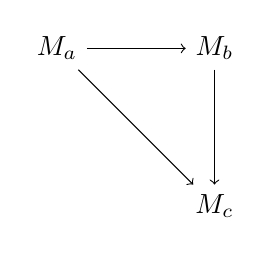
\begin{tikzpicture}[node distance=2cm, auto]
        % Nodes
        \node (A) {$M_{a}$};
        \node (B) [right of=A] {$M_{b}$};
        \node (C) [below of=B] {$M_{c}$};
        
        % Arrows
        \draw[->] (A) -- (B);
        \draw[->] (B) -- (C);
        \draw[->] (A) -- (C);
    \end{tikzpicture}
    \end{center}
    \parbox{\textwidth}{
        However, if the Hilbert manifold \(M\) has a Fredholm structure, then we can construct a direct limit C*-algebra by choosing an appropriate countable sequence \(\{M_{n}\}_{n=k}^{\infty}\) of expanding, topologically closed, finite-dimensional submanifolds of \(\operatorname{dim}(M_{n}) = n\). The sequence \(\{M_{n}\}_{n=k}^{\infty}\) is called a Fredholm filtration of \(M\) (see {\color{blue}\cite{higson1992}}).
    }
\end{frame}
%-----------------------------------------------------------------
%Highlighting text
\section{Instantly}
\begin{frame}
\frametitle{In a general sense}
In these slides, some important text will be
\alert{highlighted} because it's important.

\begin{block}{Remark}
For Fredholm manifolds \( M \), C*-algebras \( \mathcal{A}(M) \) encode the structure of \( M \) in infinite dimensions.
\end{block}
\pause
\begin{alertblock}{Theorem} 
For a Fredholm manifold \( M \) with a Fredholm filtration, the direct limit C*-algebra \( \mathcal{A}(M) \) exists and encodes \( M \)'s infinite-dimensional structure (see {\color{blue}\cite{higson2001}}).
\end{alertblock}
\pause
\begin{examples}
For \( M \) = \( E^{2} \), the C*-algebra is \( C_{0}(E^{2}, \operatorname{Cliff}(E^{2})) \) (see {\color{blue}\cite{trout1984}}).
\end{examples}
\end{frame}
%---------------------------------------------------------
\section{Objectives}
\begin{frame}{Objectives}
    \parbox{\textwidth}{
        The primary objectives of this research are:
        \begin{itemize}
            \item Investigate the construction of C*-algebras associated with infinite-dimensional Hilbert manifolds, leveraging Fredholm structures and Fredholm filtrations.
            \item Explore the application of Clifford C*-algebras and the Thom *-Homomorphism to characterize topological and geometric properties of these manifolds.
            \item Develop a comprehensive understanding of K-theory for such infinite-dimensional spaces, focusing on the relationship between C*-algebras and topological K-theory.
            \item Establish connections between noncommutative geometry and the study of infinite-dimensional manifolds through C*-algebraic techniques (see {\color{blue}\cite{tromba1988}}).
        \end{itemize}
    }
\end{frame}
%---------------------------------------------------------
\section{Conclusion}
\begin{frame}{Conclusion}
    \parbox{\textwidth}{
        This research plan outlines a systematic approach to investigate the construction and properties of C*-algebras associated with infinite-dimensional Hilbert manifolds. By leveraging the theory of Fredholm manifolds and advanced algebraic techniques, we aim to deepen our understanding of the interplay between geometry, topology, and operator algebras in the infinite-dimensional setting.
    }
\end{frame}
%---------------------------------------------------------
\section{References}
\begin{frame}[allowframebreaks]{References}
    \printbibliography
    \hyperlink{titlepage}{\beamergotobutton{Go to Title Page}}
\end{frame} 
\end{document}